%%
%% This is file `sample-authordraft.tex',
%% generated with the docstrip utility.
%%
%% The original source files were:
%%
%% samples.dtx  (with options: `authordraft')
%% 
%% IMPORTANT NOTICE:
%% 
%% For the copyright see the source file.
%% 
%% Any modified versions of this file must be renamed
%% with new filenames distinct from sample-authordraft.tex.
%% 
%% For distribution of the original source see the terms
%% for copying and modification in the file samples.dtx.
%% 
%% This generated file may be distributed as long as the
%% original source files, as listed above, are part of the
%% same distribution. (The sources need not necessarily be
%% in the same archive or directory.)
%%
%% The first command in your LaTeX source must be the \documentclass command.
% \documentclass[sigconf,authordraft]{acmart}
\documentclass[sigconf]{acmart}

\settopmatter{printacmref=false} % Removes citation information below abstract
\renewcommand\footnotetextcopyrightpermission[1]{} % removes footnote with conference information in first column
\pagestyle{plain} % removes running headers


\usepackage[noorphans,indentfirst=false,leftmargin=1em,vskip=0.5ex]{quoting}
\usepackage{microtype}

\newcommand{\pr}[1]{\textsc{pr}\oldstylenums{#1}}

%% NOTE that a single column version may required for 
%% submission and peer review. This can be done by changing
%% the \doucmentclass[...]{acmart} in this template to 
%% \documentclass[manuscript,screen]{acmart}
%% 
%% To ensure 100% compatibility, please check the white list of
%% approved LaTeX packages to be used with the Master Article Template at
%% https://www.acm.org/publications/taps/whitelist-of-latex-packages 
%% before creating your document. The white list page provides 
%% information on how to submit additional LaTeX packages for 
%% review and adoption.
%% Fonts used in the template cannot be substituted; margin 
%% adjustments are not allowed.

%%
%% \BibTeX command to typeset BibTeX logo in the docs
\AtBeginDocument{%
  \providecommand\BibTeX{{%
    \normalfont B\kern-0.5em{\scshape i\kern-0.25em b}\kern-0.8em\TeX}}}


\setcopyright{none}
\acmConference[]{}{}{}




\begin{document}

\title{Students’ Views on Adapting Computing to Climate Change}

\author{\textsc{hcin}600 group 4}
\affiliation{%
  \institution{Rochester Institute of Technology}
  \city{Rochester}
  \state{New York}
  \country{USA}
}

% \author{Narayanan Asuri Krishnan}
% \affiliation{%
%   \institution{Rochester Institute of Technology}
%   \city{Rochester}
%   \state{New York}
%   \country{USA}
% }
% \email{nk1581@rit.edu}

% \author{Xin Miao Lin}
% \affiliation{%
%   \institution{Rochester Institute of Technology}
%   \city{Rochester}
%   \state{New York}
%   \country{USA}
% }
% \email{xl3439@rit.edu}

% \author{Caluã de Lacerda Pataca}
% \email{cd4610@rit.edu}
% % \authornote{All authors contributed equally to this research.}
% \affiliation{%
%   \institution{Rochester Institute of Technology}
%   \city{Rochester}
%   \state{New York}
%   \country{USA}
% }

% \author{Yuting Shao}
% \affiliation{%
%   \institution{Rochester Institute of Technology}
%   \city{Rochester}
%   \state{New York}
%   \country{USA}
% }
% \email{ys2884@rit.edu }

% \author{Xiaoyin Xi}
% \affiliation{%
%   \institution{Rochester Institute of Technology}
%   \city{Rochester}
%   \state{New York}
%   \country{USA}
% }
% \email{xx4455@rit.edu}

%%
%% By default, the full list of authors will be used in the page
%% headers. Often, this list is too long, and will overlap
%% other information printed in the page headers. This command allows
%% the author to define a more concise list
%% of authors' names for this purpose.
\renewcommand{\shortauthors}{Group 4}

%%
%% The abstract is a short summary of the work to be presented in the
%% article.
\begin{abstract}
Scelerisque faucibus velit tincidunt ad conubia parturient conubia suspendisse lobortis sit facilisis phasellus parturient vestibulum sed scelerisque a condimentum in amet a fames a maecenas taciti. A in ultrices ullamcorper ipsum molestie adipiscing inceptos scelerisque parturient vitae vel sodales dignissim porta a a ad risus adipiscing suspendisse nascetur metus eu viverra egestas a condimentum in. Condimentum ullamcorper placerat sem vestibulum pharetra ad habitasse at consectetur sem cursus scelerisque pulvinar ornare. Nam quisque consectetur netus mollis elementum pharetra inceptos parturient a ultrices sapien nibh mollis luctus a adipiscing turpis a eu id vestibulum a sociosqu.
\end{abstract}

%%
%% The code below is generated by the tool at http://dl.acm.org/ccs.cfm.
%% Please copy and paste the code instead of the example below.
%%
% \begin{CCSXML}
% <ccs2012>
%  <concept>
%   <concept_id>10010520.10010553.10010562</concept_id>
%   <concept_desc>Computer systems organization~Embedded systems</concept_desc>
%   <concept_significance>500</concept_significance>
%  </concept>
%  <concept>
%   <concept_id>10010520.10010575.10010755</concept_id>
%   <concept_desc>Computer systems organization~Redundancy</concept_desc>
%   <concept_significance>300</concept_significance>
%  </concept>
%  <concept>
%   <concept_id>10010520.10010553.10010554</concept_id>
%   <concept_desc>Computer systems organization~Robotics</concept_desc>
%   <concept_significance>100</concept_significance>
%  </concept>
%  <concept>
%   <concept_id>10003033.10003083.10003095</concept_id>
%   <concept_desc>Networks~Network reliability</concept_desc>
%   <concept_significance>100</concept_significance>
%  </concept>
% </ccs2012>
% \end{CCSXML}

% \ccsdesc[500]{Computer systems organization~Embedded systems}
% \ccsdesc[300]{Computer systems organization~Redundancy}
% \ccsdesc{Computer systems organization~Robotics}
% \ccsdesc[100]{Networks~Network reliability}

%%
%% Keywords. The author(s) should pick words that accurately describe
%% the work being presented. Separate the keywords with commas.
% \keywords{climate change, collapse computing}

%% A "teaser" image appears between the author and affiliation
%% information and the body of the document, and typically spans the
%% page.
% \begin{teaserfigure}
%   \includegraphics[width=\textwidth]{sampleteaser}
%   \caption{Seattle Mariners at Spring Training, 2010.}
%   \Description{Enjoying the baseball game from the third-base
%   seats. Ichiro Suzuki preparing to bat.}
%   \label{fig:teaser}
% \end{teaserfigure}

%%
%% This command processes the author and affiliation and title
%% information and builds the first part of the formatted document.
\settopmatter{printfolios=true}
\maketitle

\section{Introduction}

As its harsh realities spread %dizzyingly 
over everyday life, climate change has become a dominant theme in societal discourse. While discussions about the extent of the damage already done, our shared future prospects, and possible mitigation strategies are still a highly politically charged topic, even traditionally denialist blocs have started acknowledging that \emph{something} must be done \cite{teirstein_2021}.  

In computing, the discussion about how the field is related to and could act on climate change is not new but has become more prominent in recent years. Considering scholarly work, for instance, in the \textsc{acm} Digital Library there were \oldstylenums{295} climate change-related papers published between \oldstylenums{1991} and \oldstylenums{2009}, with another \oldstylenums{2,095} then published from \oldstylenums{2010} to \oldstylenums{2020} \cite{ferreiraClimateChangeCommunication2021}. As a complex, multi-variate issue, different researchers have adopted varied approaches about what role computing should play. \citet{easterbrook2010climate}, for example, argues that the software community has to ``step up to the plate,'' as other fields have done, and calls for a discipline-wide effort on work on software to ``support the science of understanding climate change[,] to support the global collective decision making[, and] to reduce the carbon footprint of modern technology.''

This fits what \citet{silberman2010precarious} call \emph{adaptation-oriented pre-apocalyptic computing}, which assumes a future apocalypse\footnote{The term, which the authors acknowledge as perhaps too \emph{inflammatory} for scholarly use, ``denotes an event in the intersection of the spaces of events denoted by the terms \emph{collapse} and \emph{disaster}.''} is likely, but attempts to ``develop tools for users to negotiate it successfully,'' making it ``less apocalyptic [with] materials and social relations available at design time (pre-apocalypse) but likely to be unavailable at use time.'' An alternative approach, \emph{adaptation-oriented post-apocalyptic computing} works within material constraints as if the apocalypse had already happened, thus anticipating and easing a transition towards future conditions --- which, interestingly, makes this approach share methods with the already-present realities of ``disaster informatics, community informatics, \textsc{ict\oldstylenums{4}d}, \textsc{hci\oldstylenums{4}d}, humanitarian logistics, sociotechnical action research and `post normal science`" --- for many underdeveloped regions around the world, the ``ingredients of apocalyptic computings and other related practices [constituting] deindustrial techne'' are are already a given.

In that vein, \citet{nardiComputingLimits2018} challenge computing's assumed premise that ``exponential growth of computing capacity and an ever-expanding infrastructure for computing will continue into the future,'' positing that, as world-limits make themselves felt, an alternative, and even optimistic, approach would be to strive for a ``transformative change to a system more like steady-state economy,'' i.e. one not predicated on continuous economic (and resource consumption) growth. 
\citet{wong2009prepare} goes further: in denouncing how designers ``often confuse needs with desire,'' they claim that designers ``will need to recognize the pervasiveness and insidiousness of denial in materialistic populations,'' and that perhaps a reality shock (brought upon a collapse of much of what makes present-day computing possible) will allow sustainable interaction design to ``shift its focus from persuading to sustaining the human race.''

All of this begets the question: how is the new generation of computing professionals readying themselves to act within this scenario that, while bleak, will inevitably shape their future careers? While climate change affects the field as a whole, new and old professionals alike, we chose to focus on computing students since their mental models about computing's role in the Anthropocene are supposedly still being shaped by their on-going education. This, we posit, might give a good indication of where the field is heading. This study attempts to answer the following research questions:

\begin{enumerate}
    \item If students feel that climate change will impact how their field of expertise works?
    \item If they do, what do computing students think their field of expertise will look like during the effects of climate change?
\end{enumerate}


\section{Methods}

% We should probably cite \citet{braun2006using} here...
We aim to understand perceptions of computer science students about climate change and how their field affects and is affected by it. To gauge these opinions, we conducted 5 semi-structured interviews with students varying from undergraduate and graduate levels. In this section we describe how we collected the data, extracted themes and deduced results from the data.

\subsection{Materials and Procedure}
The semi-structured interview included \oldstylenums{13} questions that are tailored to provide insights for our research questions. Q1-Q5 collected demographic information on participant name, gender, age and area of expertise. Q6 was a general warm-up question about the participant’s professional plan for the future. Q7-Q9 were used to answer “How climate change was perceived in daily life?”. Q10-Q11 aimed to find out “How climate change would influence their area of expertise?”. Q12-Q13 discovered “What opportunities were presented in terms of alleviating the effects of climate change?”. 

There were a total of \oldstylenums{5} interviews conducted. The interviews were all semi-structured and most questions came from the interview guide that was made explicit above. There were other follow-up questions raised depending on the answers of the interviewee during the interview process. The interviews were conducted online using a video messaging platform called Zoom and all of them lasted around \oldstylenums{20} minutes each. The interviews were recorded with permission and transcribed afterwards. 

% \footnote{https://zoom.us/}

\subsection{Analysis}
After conducting and transcribing the interviews, we analyzed them using a bottom-up, inductive process, as per \citet{braun2006using}.

\subsubsection{Generating and collating initial codes} Interviews were bundled into one document. Each author was given a copy of this final transcript and annotated them individually without communication or interference from other authors, extracting initial codes from the interviews. After being generated, they were collated and collapsed by the similarity of their content, then displayed as sticky notes using a collaborative whiteboard platform.
% called Miro \footnote{https://www.miro.com}. %Figure \ref{fig:initial-codes} shows an example of initial codes created by one of the authors.

% \begin{figure}
%     \centering
%     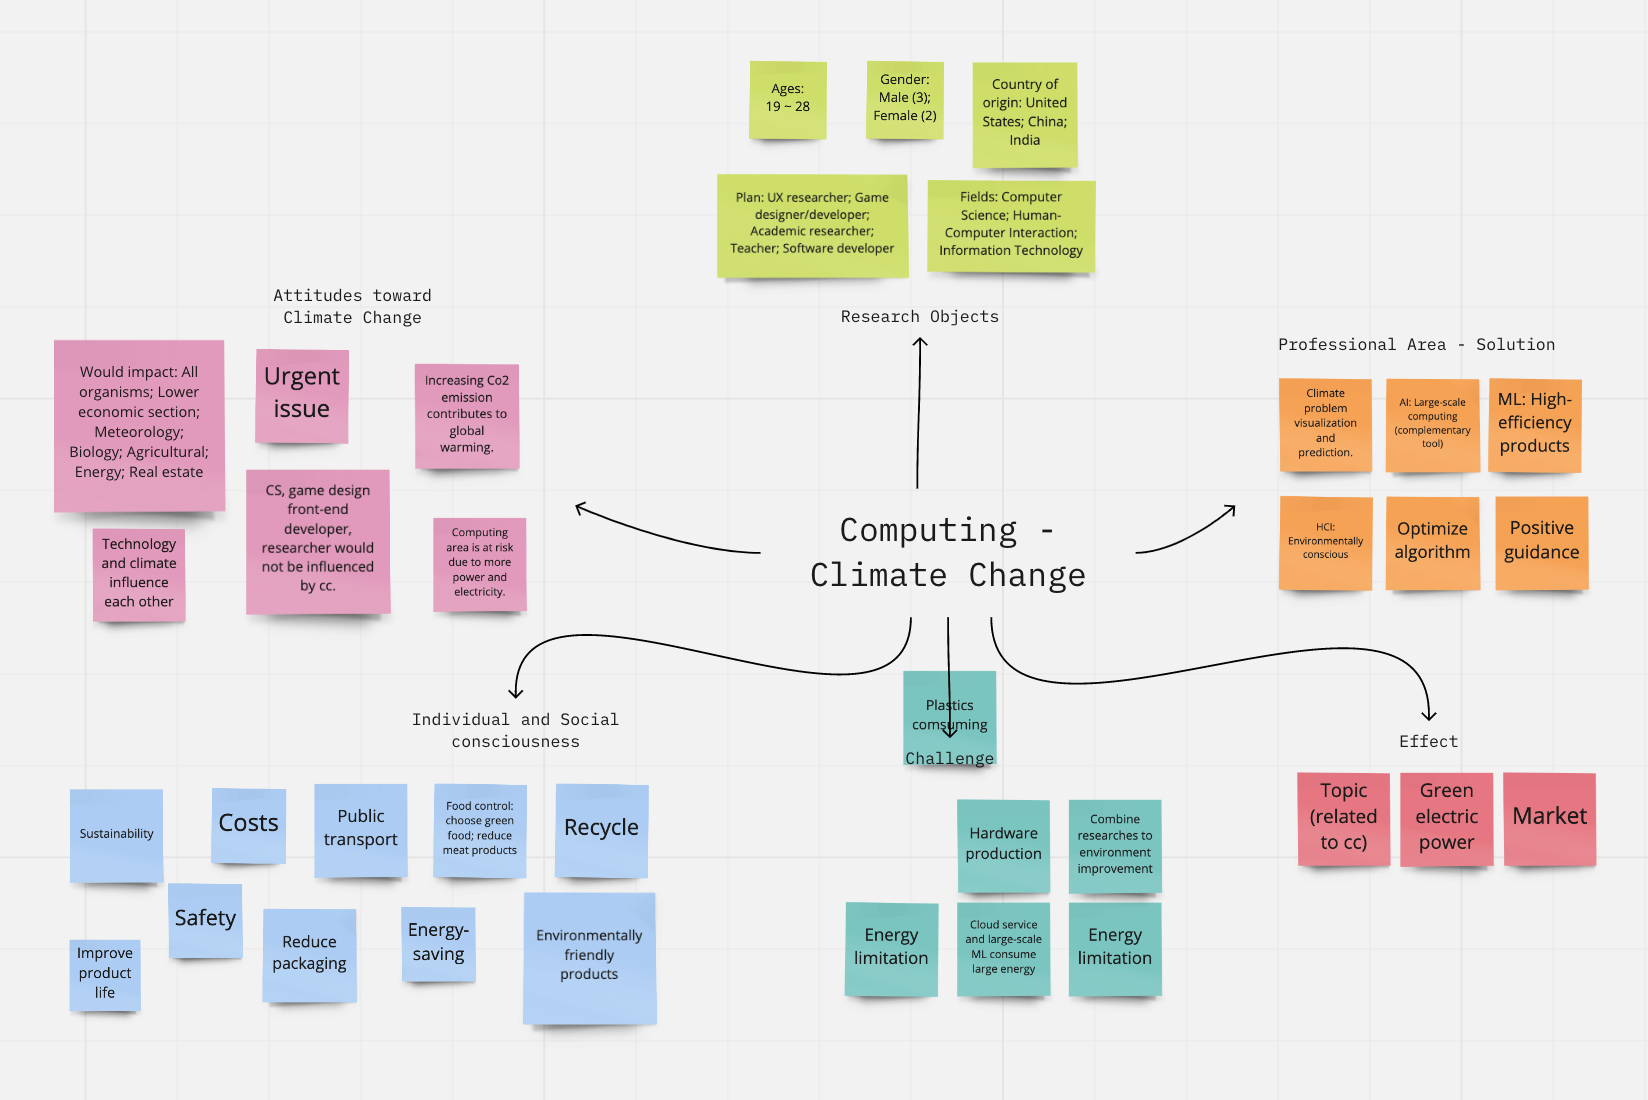
\includegraphics[scale = 0.2]{Figures/Initial Codes.png}
%     \caption{Example of Initial Codes}
%     \label{fig:initial-codes}
% \end{figure}

\subsubsection{Defining themes}

After pasting all codes in the same place, we created an overall coding diagram to identify similarities that allowed thematic grouping. We ended up identifying four major categories, to which we attached the codes' post-its. %Figure \ref{fig:theme-codes} illustrates this process. 
All four categories provide insights to our research questions for the ``perception of climate change'' and the ``impact on area of expertise.'' Finally, in writing the report, we created the final two themes, \emph{Unsystematic risks} and \emph{Limits to action}, with which we wrote our final analysis.

% \begin{figure}
%     \centering
%     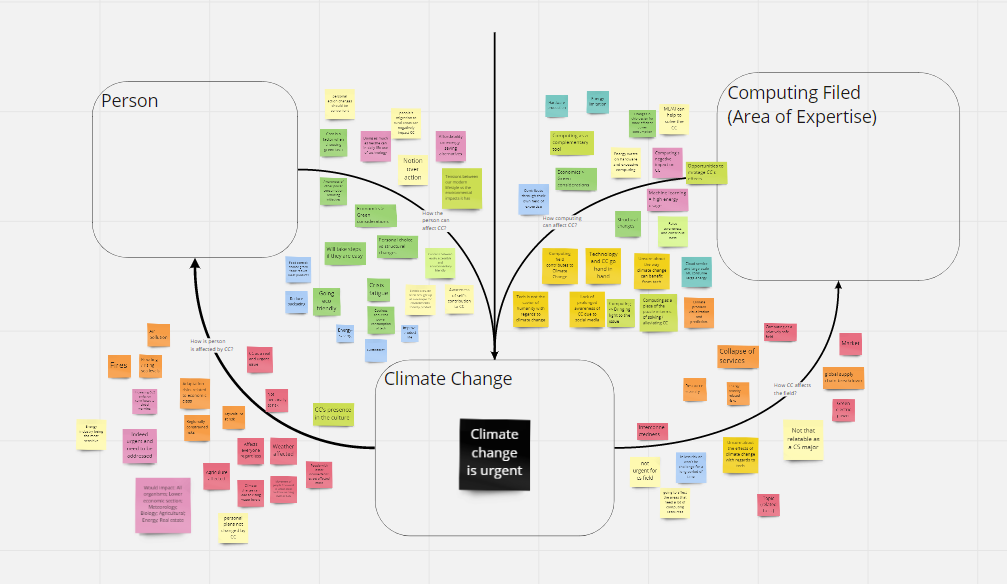
\includegraphics[scale = 0.2]{Figures/codes.png}
%     \caption{Themes and their corresponding codes}
%     \label{fig:theme-codes}
% \end{figure}



\section{Results}

\emph{(Participants' names coded for anonymity, and their responses edited for clarity and brevity.)}

    \subsection{How are individuals affected by Climate Change?}
    
    \begin{quoting}
        \textit{``It's affecting everybody, it affects humans, animals, at the end of the day, the tech field are still people who get adversely affected by climate, right? So honestly, I don't know if there is a demarcation between tech people and non-tech people when it comes to climate change, it just affects everybody regardless.''} (\pr{1})
    \end{quoting}

    From the interviews, it is observed that the all the participants believe that climate change is urgent and needs to be planned for. \pr{1} mentions that although the effects of climate change will be seen on the tech field, it is not isolated to the tech field and should be considered as a global problem.
    
    \begin{quoting}
        \textit{``Also, I mean, I was listening to this podcast, I think it is called `How to change the world'... it's a climate podcast, and one of the episodes was about the rising… It was about Miami, and how the sea level continues to rise, and how they are just building, you know, they continue to elevate their buildings and, no one really talks enough about how this is an issue, you know, we can't keep putting our buildings on stilts.''} (\pr{2})
    \end{quoting}
    
    \begin{quoting}
        \textit{``Particularly sensitive to climate change I would think of the energy field. Fossil fuels are a big part and climate change. I would also add real estate, because if the ice caps melt and the sea levels rise as you're seeing in some places already, those beach side properties will be underwater.''} (\pr{4})
    \end{quoting}

    \begin{quoting}
        \textit{``Actually, I think in city it is also urgent or sensitive, because as more and more people are moving from rural areas to cities, this will increase CO\textsubscript{2} emissions, which is one of the major causes for the global warming.''} (\pr{5})
    \end{quoting}
    
    \begin{quoting}
        \textit{``I think the lower economic section gets affected by it more, but the upper economic section can reduce the impact of climate change for themselves. For example, if you are a very rich farmer, you can get irrigation or better seeds, but if you are a poor farmer and the rains are not on time because of climate change, then you are in a bad position.''} (\pr{1})
    \end{quoting}

    All participants agree that there are certain areas that are more sensitive and will be affected adversely by climate change. \pr{2} and \pr{4} talk about the melting icecaps and rising water levels in the oceans and how this is problem for cities built on the coast. \citet{hitz2004estimating} illustrate the rising sea levels will cause loss of land, larger damages from storms, saltwater intrusion and increased cost in coastal defenses. \pr{5} feels that due to the migration of citizens from rural to urban areas there will be an increase in emission of CO\textsubscript{2}, contributing to global warming --- which, it is worth noting, is not in line with recent research on the topic. \cite{castells2020density} \pr{1} feels that rather than only looking at the effects from a global standpoint, we must also look at them for groups from lower economic backgrounds, who will be less prepared for the effects of Climate Change.
    
    \begin{quoting}
        \textit{``I mean, I feel like I don't personally fear for myself getting, you know… I am not worried about [whether] where I live down there is going to catch on fire''} (\pr{2})
    \end{quoting}

    While most participants talked about how the drastic change in climate would affect the population of earth, they did not mention how these changes would personally affect them. \pr{2} did mention that although they were concerned about the effects of climate change, they felt that it would not personally change their plans.
    \subsection{How individuals can affect Climate Change}
    
    Our interview participants all acknowledged that climate change is indeed an urgent issue and can to addressed through both monitoring individually daily usage of technology and raising awareness of power consumption of certain computing fields. However, there are challenges to adopt a more environmentally friendly lifestyle.
    
    \subsubsection{Individual Behavior Changes}
    
    Several participants express the intention to incorporate personal behavior changes to combat climate change. It's worth noting that electric cars are often mentioned as something they would considering purchasing:
    
    \begin{quoting}
        \textit{``I'm becoming more conscious about the power that tech uses. For example, I used to leave my PlayStation on rest mode, but now I power it off. I know it's not much, but if a million people started doing it, that's a big deal.''} (\pr{1}) % as it only uses about 4 watts per hour
    \end{quoting}
    
    \begin{quoting}
        \textit{``I may change my private car to energy-saving and environment-friendly in the future. Electric cars are a good choice.''} (\pr{3})
    \end{quoting}
    
    % Concerns over transferring to electric vehicles were also brought up by one participant.

    \begin{quoting}
        \textit{``I've read suggestions of using your current appliances till the end of their lifespan, and to then recycle them, avoiding byproducts that would harm the environment. For instance, I plan on buying an eclectic car or hybrid in the future, but I'll drive my current car until it is no longer operable.''} (\pr{4})
    \end{quoting}
    
    One participant mentioned that structural change should be more emphasized in term of impact on climate change:
    
    \begin{quoting}
        \textit{``I do not think that the everyday use of technology will change much, but those big companies that consume a lot of plastics [will have to change].''} (\pr{5})
    \end{quoting}
    
    \subsubsection{Challenges of changing lifestyles}
    
    While most participants stated that they would love to adapt an environmentally friendly and energy-saving lifestyle, they also realized that such change can be unpleasant and hard to execute. Affordability is the major concerns for some of our participants. %Partly due to the demographic distribution in our research, 
    
    \begin{quoting}
        \textit{``I would say that I couldn't afford an electric car right now, but that would be an ideal plan.''} (\pr{2})
    \end{quoting}
    
    \begin{quoting}
        \textit{``It again comes down to the trade-off, because the greener the tech you want right now, the more expensive it gets. Very weird situation but unfortunately that's what it is. If it's within budget, or even if it's reasonably above budget, then I would go for a greener option, but yeah at the end of the day it comes down to economics.''} (\pr{1})
    \end{quoting}
    
    The tension between a comfortable lifestyle versus an inconvenient and expensive but environmentally friendly one is present in many participants' answers. %what cause people's hesitation of the change
    
    \begin{quoting}
        \textit{``We're so used to having everything accessible within days or hours. I can order something from across the country and it'll be here in two days, and I can do that through an app, through the click of my fingers, and I think that's something that… you know, as someone who's in the field of user experience, and making things easier for users, I think, sure, we want to make things easy for users, and accessible, but I feel like we also don't want to neglect being environmentally conscious, and we don't want to make things too easy that we are lazy and neglectful''} (\pr{2})
    \end{quoting}

    
\subsection{How are computing fields can affect Climate Change}

    % This results section is spread out according to two progressive core questions.
    
    % \subsubsection{Interview Question: Do you feel your specific field presents unique opportunities in terms of alleviating the effects of climate change? And how impactful do you think they could be?}
    
    Many participants believe their own computing field of expertise can both worsen and help alleviate climate change's effects: %, especially advantage in large-scale computing.
        
    % \begin{quoting}
    %     \textit{
    %     "[The] problem can be visualized and predicted, based on existing receipts generated images and analysis." (\pr{3})
    %     }
    % \end{quoting}
    
    \begin{quoting}
        \textit{
        ``As we know that all [of the effects of] climate change can be recorded in the database, if we want to get more useful information, we cannot ignore the powerful tools of the AI.''       }(\pr{5})
    \end{quoting}
    
    \begin{quoting}
        \textit{
        ``There is a lot of room where we can optimize (looking to optimize power efficiency in data centers). There are a lot of industries where ML and AI could help.''
        }  (\pr{1})
    \end{quoting}
    
    \begin{quoting}
        \textit{
        ``I think that [games] would let people be more conscious about how they affect the climate.''
        }(\pr{4})
    \end{quoting}
    
    One participant reported their ambiguous and confused attitude when considering the field of user experience:
    
    \begin{quoting}
        \textit{
        ``We want to make things easy and accessible for users, but I feel like we also don't want to neglect being environmentally conscious, and we don't want to make things too easy that we are lazy and neglectful. I definitely will order things from Amazon, and I'm like, `that's probably not the best thing to do. Why don't I just go outside of my apartment, walk down the street and buy things locally?'\thinspace''  % Which are things that have become more.
        }(\pr{2})
    \end{quoting}
    
    \begin{quoting}
        \textit{
        ``When I was an undergrad [in architecture], the topic of climate change was very much in my everyday language, and since taking the \textsc{hci} path, it kind of lost it a bit...''        }(\pr{2})
    \end{quoting}
    
    Some participants also reported the negative effects that computing has on climate change. Most of these concerns were related to large-scale energy consumption:
    
    \begin{quoting}
        \textit{
        ``[Cloud services] need to consume a tremendous amount of energy and, to maintain operating speed, additional power is needed to dissipate heat.''
        } (\pr{3})
    \end{quoting}
    
    \begin{quoting}
        \textit{
        ``For some research doing large-scale machine learning, they will use a lot of electricity[, and] their long-term goals are not aligned with a green climate trend.'' (\pr{5})
        }
    \end{quoting}
    
    % Further, discussed how impactful computing could be for alleviating the effects of climate change. 
    
    Some participants mentioned that even though computing brings light to the climate change issue, it is just a piece of the puzzle in terms of solving climate change. For example, one participant considered that, in most cases, technology could be just a complementary tool. Another participant reported that what current computing can do is to make small and minor improvements. %And depending on the scale, it will make a difference.
    
    Meanwhile, some participants kept uncertain attitudes. For example, one participant mentioned that social media impacted people to a big degree, but they were not sure about the level of influence of social media could have specifically on climate change:
    
    \begin{quoting}
        \textit{
        ``[In the] computer field, our advantages are very strong social communication and influence. But depending on past experience, good media tend to spread [virally]. However, we won't know how people will behave after transmission.'' 
        }(\pr{3})
    \end{quoting}
    

\section{Discussion}

\subsection{Unsystematic risks}

All participants were unanimous in stating that they felt climate change as a real and urgent issue. In their understanding of the scope of the risks posed by it, however, its effects were generally perceived as if of an unsystematic nature, in line with what \citeauthor{silberman2010precarious} call \emph{emergencies}, i.e., ``events that have impacts on social units, which mobilize responses to these impacts,'' but which do not usually \emph{exceed} society's capabilities for response.

This is seen both in how they imagine themselves potentially affected by climate change and how they feel the computing field will (if at all) change in response to it. \pr{2}, for instance, knows that Albuquerque, New Mexico (where they plan to move to), is suffering from out-of-control wildfires and an on-going major drought. Yet, these are seem as inconveniences but not necessarily deal-breakers.

While there were hints of how parts of computing are interconnected --- e.g. \pr{4} saying that ``if you were working with hardware [and you could not get the resources because] they would be shutting down the plant'' ---, the more general perception is that there are certain \emph{localized} risks that could cause disruptions, but not a \emph{collapse}. The societal status quo is seen as inherently stable.

In this sense, participants seem to call for a loose \emph{adaptation-oriented pre-apocalyptic computing} within a very limited scope. They propose specific changes, both for the field and their personal lives, but these are discontinuous and, more especially, non-structural: on a personal level, many mentioned wanting to change an \textsc{ice} car for an electric one, but there was little discussion of car-dependency embedded in city design; in computing, there was mention of the use of green components in computer manufacturing, but consumerism itself was only briefly mentioned.

\pr{2} hinted at this contradiction between how limits to what non-structural changes are capable of achieving when they pointed that convenience, as it is embedded in everyday apps and services, is contradictory with environmentalism, an apparently unsolvable conundrum since ``companies should not make bad apps.''

\subsection{Limits to action}

A second theme we perceived in participants' answers was that they seemed to see themselves as if helpless to initiate any major changes, be it societal or in their own fields of expertise. Not only did they generally avoid discussing the need for structural changes, what changes they did suggest or see as forthcoming are all implicitly initiated by unknowable forces, over which the interviewees seem to have no say.

This, again, seems to be tied to a notion of climate change-related risks as if geographically and chronologically far off, and to the belief that whatever society emerges from it will be a superficially improved but structurally similar version of ours.

Even if one assumes, like \citeauthor{easterbrook2010climate}, an \emph{adaptation-oriented pre-apocalyptic computing} scenario, mitigation is necessarily a costly endeavor and one which needs careful coordination and intense effort. In this case, this passivity is worrying, as it seems to indicate that reflections about climate change are still superficial.

It also worrying when one considers that, if \emph{collapses} do occur, current students might be ill-equipped to adapt to new circumstances. If, as states \citeauthor{wong2009prepare}, ``our future lacks some of the technology opulence we have grown to expect, there are still plenty of opportunities for sustainable interaction design to have an impact,'' it would seem important to explore some of these opportunities at our present \emph{pre-apocalyptic} context.




\subsection{Limitations of this study}
For one, time restrictions limited our number of interviewees to only \oldstylenums{5}. While we were able to obtain a varied set of responses, sub-fields of computing were underrepresented, when at all, i.e., we only had one participant from \textsc{hci}, one from game development, etc. Considering how \cite{easterbrook2010climate} proposes sub-field related responses, a broader and more representative sample could deepen the discussion of more specific educational interventions, for instance.

The small sample also meant that we did not achieve data saturation, so while there were common themes between participants' responses, there was also a lot of variety among them. Given our decision to design a short interview guide, more participants could increase confidence in our thematic analysis.

\section{Conclusions and Future work}
As a way to potentially help the debate about how the computing field can evolve to better deal with climate change, and also as a query into how its next generation of practitioners imagine the field will change in the coming years, our research interviewed computing students from different educational levels. 

We asked them about their perceptions about the interactions between the field and climate change. In response to our first research question (\emph{if they feel that climate change will impact how their field of expertise works?}), the general answer seems to be that yes, the field will change, even if the extent to which this is perceived as true seems to be quite limited, and it is not clear to our participants who should initiate these changes. 

This feeds into our second research question (\emph{what do computing students think their field of expertise will look like during the effects of climate change?}), for which our answers pointed to a field that is only superficially different than its present state.

These answers are worrying for two reasons. First, they indicate that, even if climate change is named as an urgent matter, computing seems to have a passive attitude towards it, both in terms of protecting itself against probable disastrous future scenarios and in terms of helping society to avert them. 

Second, the answers also show that these students themselves might be receiving an education that aims an each day more unlikely future professional landscape, while at the same time ignoring steps they could be taking now to prepare themselves for this \emph{post-apocalyptic computing}, to use \citeauthor{silberman2010precarious}'s term.

Given these bleak findings, it is urgent that climate change adaptation is given a greater role in computing courses. This could be through a greater emphasis in topics like those mentioned by \citeauthor{silberman2010precarious}, \citeauthor{easterbrook2010climate}, among others. 

\subsection{Future work}


\subsection{Limitations of this study}
For one, time restrictions limited our number of interviewees to only five. While we were able to obtain a varied set of responses, sub-fields of computing were underrepresented, when at all, i.e., we only had one participant from \textsc{hci}, one from game development, etc. Considering how \cite{easterbrook2010climate} proposes sub-field related responses, a broader and more representative sample could deepen the discussion of more specific educational interventions, for instance.

The small sample also meant that we did not achieve data saturation, so while there were common themes between participants' responses, there was also a lot of variety among them. Given our decision to design a short interview guide, more participants could increase confidence in our thematic analysis.






\bibliographystyle{ACM-Reference-Format}
\bibliography{refs}

\end{document}
\endinput
%%
%% End of file `sample-authordraft.tex'.